\section{Esercizio 16}
\begin{itemize}
\item Hermite
\lstinputlisting[language=Matlab]{CodiceMatlab/Esercizio15-19/hermite.m}
\item Script es. 16
\lstinputlisting[language=Matlab]{CodiceMatlab/Esercizio15-19/scriptEs16.m}
\end{itemize}
Eseguendo lo script si ottiene il seguente grafico: 

\begin{figure}[h!]
    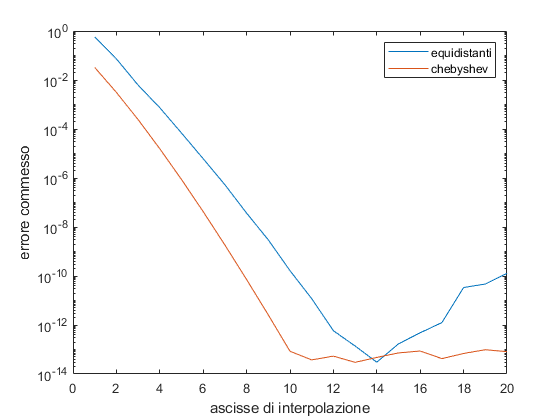
\includegraphics[scale=0.8]{CodiceMatlab/Esercizio15-19/graficoEs16.png}
    \caption{Grafico esercizio 16 con Hermite}
    \label{fig:es16}    
\end{figure}

Si può osservare che dopo n = 10  il grafico dell'errore per le ascisse di chebyshev  presenta un andamento costante. 
Per le ascisse equidistanti utilizzando il polinomio di Hermite l'errore raggiunge il valore minimo a n = 14 ed in seguito torna a salire.
Possiamo affermare che in generale l'approssimazione tramite ascisse di chebyshev è più precisa.
